\chapter{Characterization of Components and Equipment}
\label{chap:comp}

\section{R\&S Vector Network Analyzer ZNB8}
In order to gain a deeper understanding of the non-idealities of the
components which were later used for the different test setups
were characterized using a Rohde \& Schwarz Vector Network Analyzer. \\

Besides the results of the measurements of which a few a presented
in the next few sections, also important lessons about measuring were
learned. It took me about one week to be able to perform meaningful
measurements on the ZNB4 and to understand it's features.
While performing different measurements it soon became very clear then
non optimal torque while connection plugs or overbended cables
can produce notches of dozens of dBs even when using highest quality
equipment. \\
\begin{table}[h]
  \centering
  \begin{tabular}{|l|l|}
    \hline
    Frequency range & 9 kHz to 8.5 GHz \\ \hline
    Sweep speed & about 1ms for 100 points \\ \hline
    Dynamic range & up to 140 dB \\ \hline
    Power sweep range & 98 dB \\ \hline
  \end{tabular}
  \caption{Key properties of R\&S Vector Network Analyzer ZNB8}
  \label{tab:awg}
\end{table}

\section{Arbitrary waveform generator: Tektronix AWG 7122C}
\label{sec:comp_awg}
An \acrfull{AWG} was used to generate the \gls{IF} signal.
Not only because there is no transmitter available but also because of
it's flexibility. The same Matlab script used for simulations could
also call function output the baseband or the \gls{IF} signal.
The additional marker outputs could be used to trigger the oscilloscope
as well as the data acquisition process on the \gls{FPGA}.

\begin{table}[h]
  \centering
  \begin{tabular}{|l|l|}
    \hline
    Sample Rate & 12 $\text{GS}/\text{s}$, 24 $\text{GS}/\text{s}$ (interleaved) \\ \hline
    Number of analog channels & 2, 1 interleaved \\ \hline
    Analog bandwidth & 5.6 GHz \\ \hline
    Number of digital maker channels & $2 \times 2$ \\ \hline
    Vertical resolution & 8 Bit, 10 Bit when markers are disabled \\ \hline
    Maximal waveform length & 64 MS  \\ \hline
  \end{tabular}
  \caption{Key properties of Tektronix AWG 7122C}
  \label{tab:awg}
\end{table}

\section{Sivers IMA 58-63 GHz Converter FC1005V/00}
\label{sec:comp_sivers}
The most important is component in the transmission chain is the
up- and down-converter from an \acrfull{IF} to the \acrfull{RF}.
For this purpose the Sivers IMA FC1005V/00 module was used.
It consists of an independent transmit and receive path including
a horn antenna assembly, amplifiers, up-/down-mixers and a \gls{PLL}
for frequency synthesis. It is able up-/down-mix an \gls{IF}
of between 1 and 5 GHz to the \gls{RF} of 58 to 63 GHz. \\

As shown in \figref{fig:sivers} both the transmit and receive path
use two inputs (I- and Q-channel) which are then both mixed to
\gls{RF} and than fed to a $90^\circ$ hybrid coupler. \\
This results in one of the two mirror frequency to be completely canceled
if one channel is shifted by $-90^\circ$ relative to the other.
This can be done by using another $90^\circ$ hybrid coupler working on
\gls{IF} as described in \secref{sec:comp_90deg} or by using die Hilbert
transform as shown in \secref{sec:rx_rf_1}. \\
The Sivers module is build such that it transmits on the \gls{USBand}
(canceling the \gls{LSBand}) when the Q-channel is connected to the signal
$x(t)$ and the I-channel to $\mathcal{H}\{x(t)\}$. \\

There are two independent \gls{LO} for transmission and reception both using
the reference. There is an internal 10 MHz reference on the board. During
most measurements the reference was locked to same external reference as the
\gls{AWG} and \gls{ADC} to not have any frequency offsets when different
transmit and receive frequencies were used.

\begin{figure}[p]
  \centering
  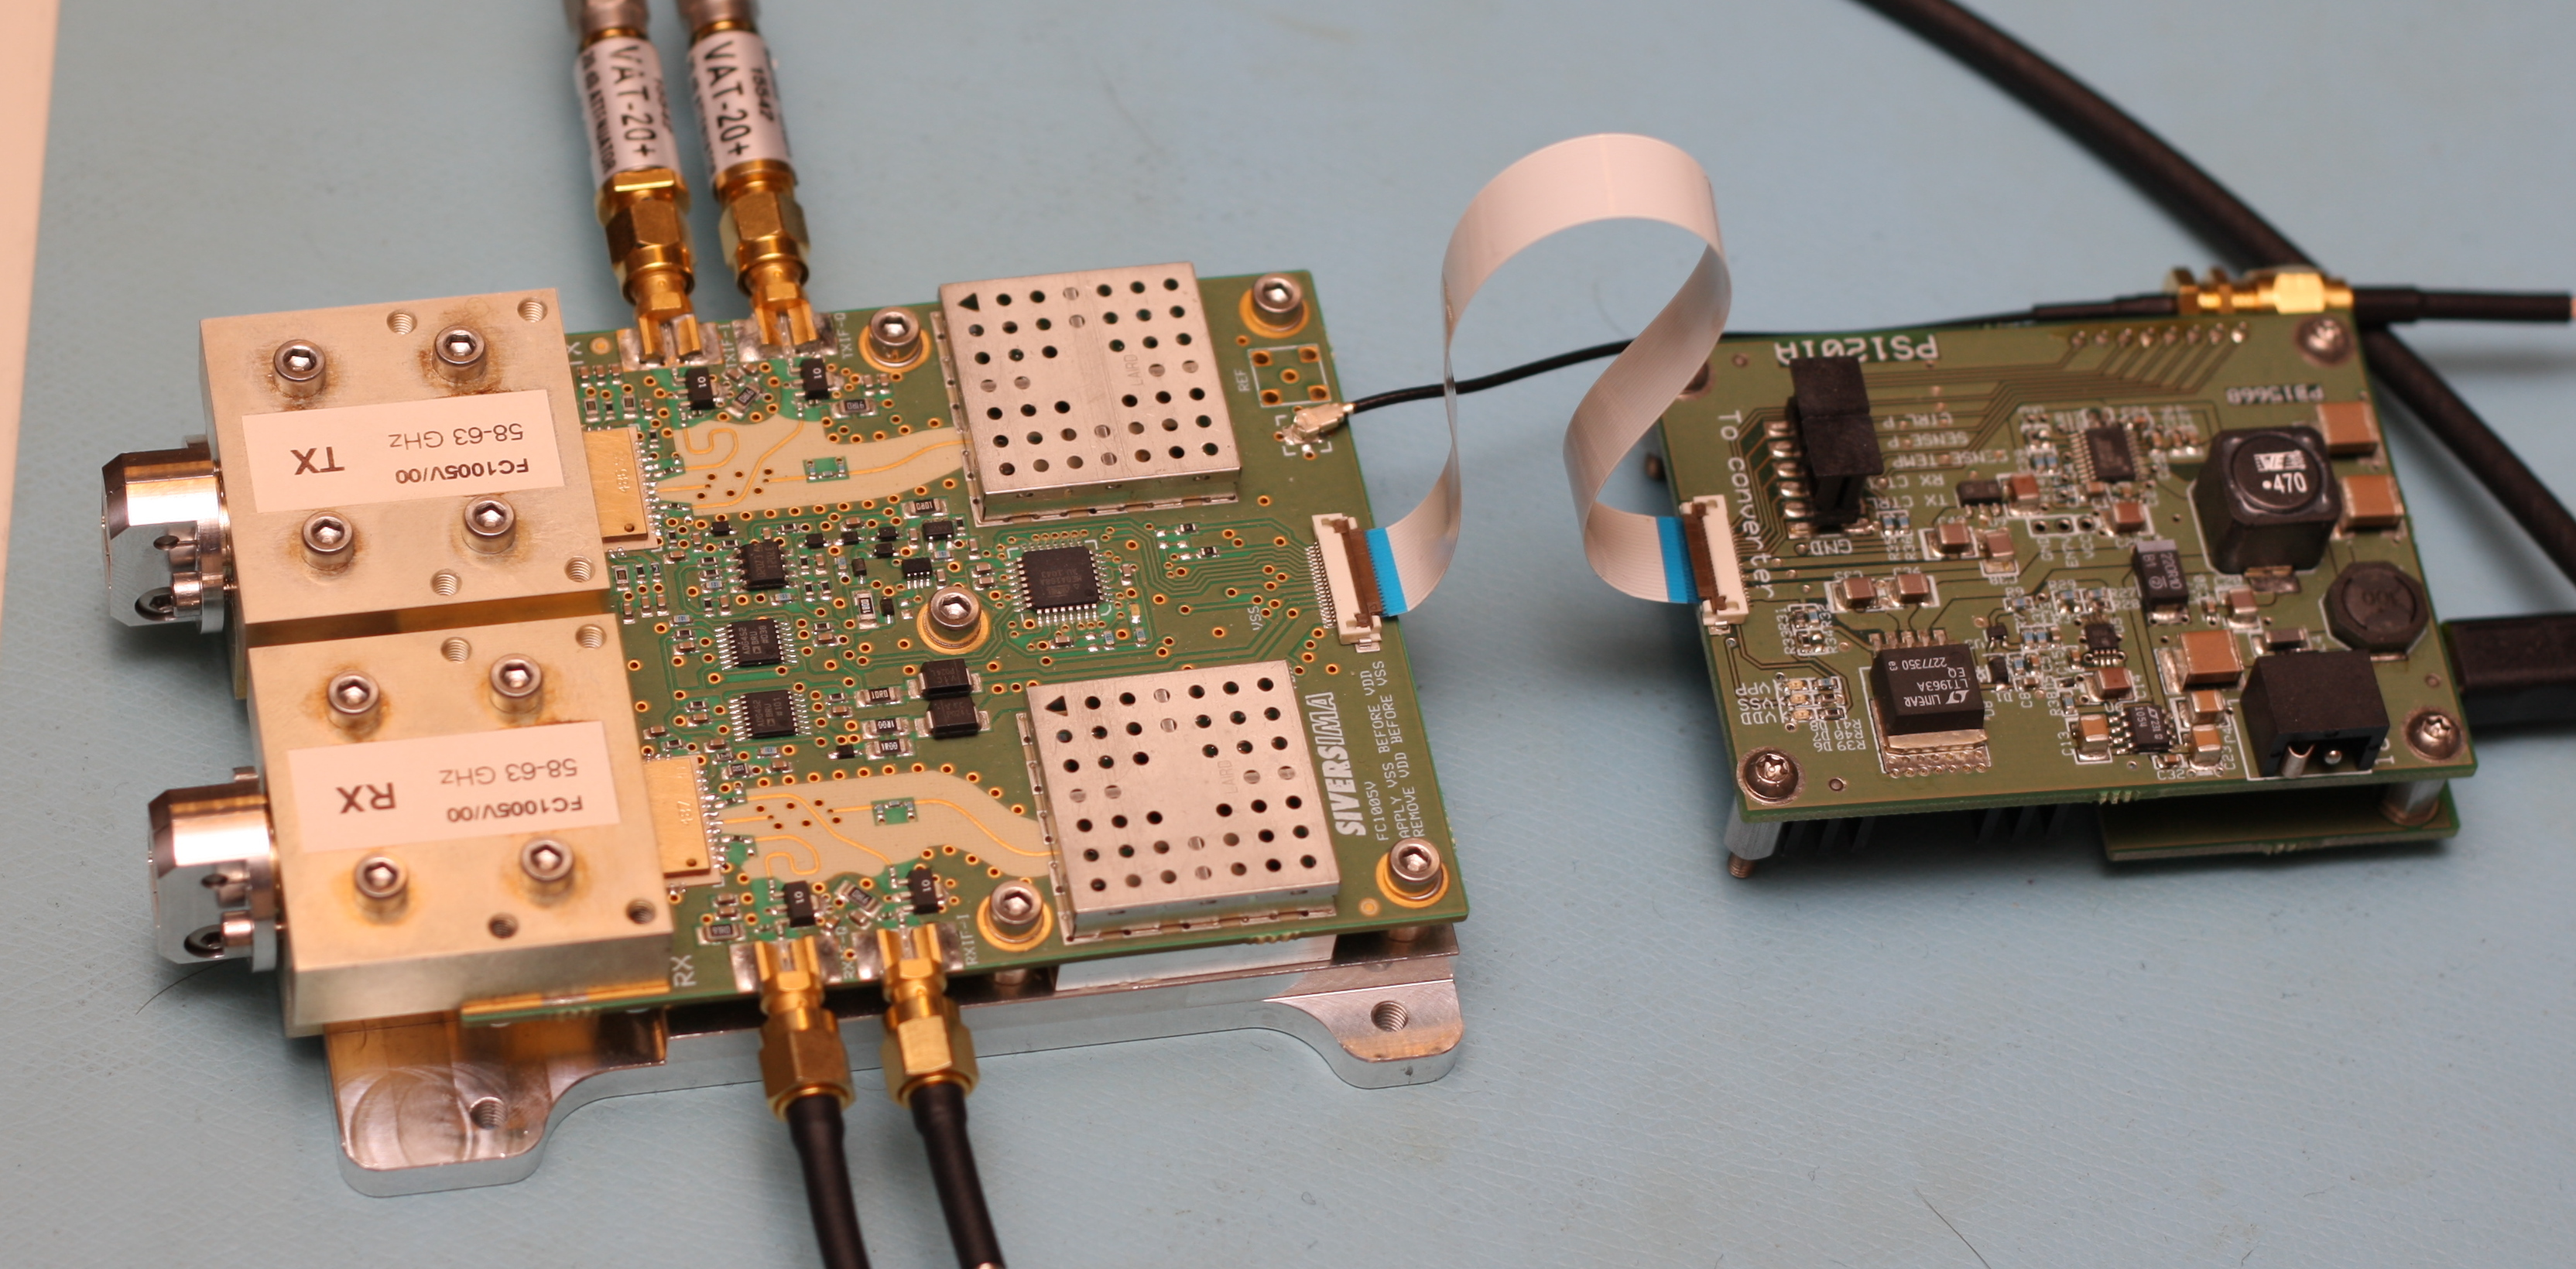
\includegraphics[width=\textwidth]{pictures/sivers}
  \caption{Picture of Sivers IMA FC1005V/00 Converter}
  \label{fig:sivers}
\end{figure}

\begin{figure}[p]
  \centering
  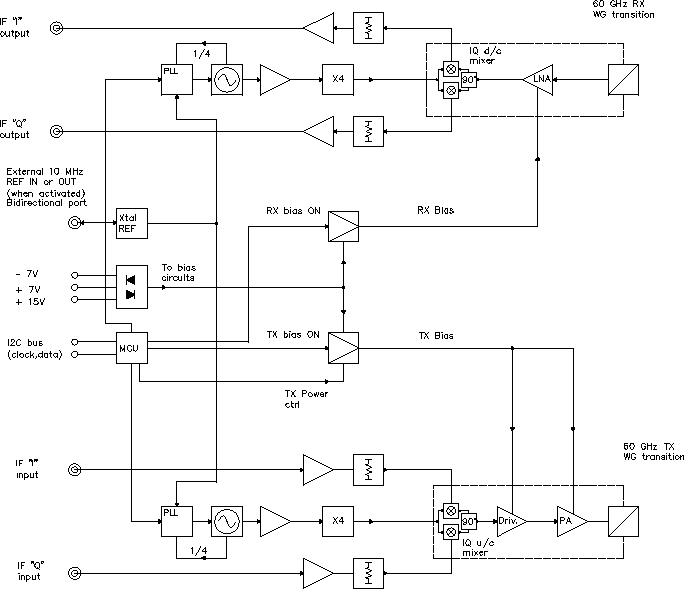
\includegraphics[width=\textwidth]{figures/sivers_block_diagram}
  \caption{Block diagram of Sivers IMA FC1005V/00 Converter \cite{sivers_fc1005v}}
  \label{fig:sivers}
\end{figure}

\begin{table}
  \centering
  \begin{tabular}{|l|l|}
    \hline
    \gls{TX} and \gls{RX} \gls{RF} range & 58 - 63 GHz \\ \hline
    \gls{TX} and \gls{RX} \gls{IF} range & 1 - 5 GHz \\ \hline
    Saturated output power & min 16 dBm \\ \hline
    \gls{LO} leakage & typical 10 dBm, max 15 dBm \\ \hline
    \gls{TX} Image rejection & min 10 dB, typical 20 dB \\ \hline
    \gls{RX} Image rejection & min 10 dB, typical 14 dB \\ \hline
    Total Power Consumption & 9.5 W \\ \hline
    1-dB output compression point & 10 dBm \\ \hline
    Nominal gain \gls{IF} to \gls{RF} & 25 - 40 db \\ \hline
  \end{tabular}
  \caption{Key properties of 58-63 GHz V-band Converter Sivers IMA FC1005V/00
    \cite{sivers_fc1005v}}
  \label{tab:awg}
\end{table}

\section{Meca 3 dB Hybrid Coupler 705S-3.000}
\label{sec:comp_90deg}

A Hybrid coupler has typically 4 ports as shown on
\figref{fig:90deg_coupler_symbol}.
One port is often 50 $\Omega$ terminated and therefor might not be connected
to a plug. \\

It is, when neglecting production imperfections, a fully symmetric component
(inputs $x_i(t)$ with outputs $y_i(t)$ as well as indices 1 and 2
can be exchanged) and has the following relations:

\begin{align}
  y_1(t) = \frac{1}{\sqrt{2}} \left[x_1(t) \angle -\frac{\pi}{2} + x_2(t) \angle -\pi \right] \\
  y_2(t) = \frac{1}{\sqrt{2}} \left[x_1(t) \angle -\pi + x_2(t) \angle -\frac{\pi}{2} \right]
\end{align}

As shown in \figref{fig:90deg_coupler_measurement} the power of
$x_1$ is not perfect equally split to $y_1$ and $y_2$. The power difference
is smaller than 1 db in the band from 1.8 GHz to 4 GHz.
Also there is a little power ($\leq -20 db$) leaking from $x_1$ to $x_2$ and from
$y_1$ to $y_2$. \\

Due to missing calibration equipment the phase rotation could not be measured.
All measured numbers matched the specifications.

\begin{figure}[p]
  \centering
  
\includegraphics{figures/90deg_coupler_symbol}
  \caption{Symbol of a $90^\circ$ Coupler}
  \label{fig:90deg_coupler_symbol}
\end{figure}

\begin{figure}[p]
  \centering
  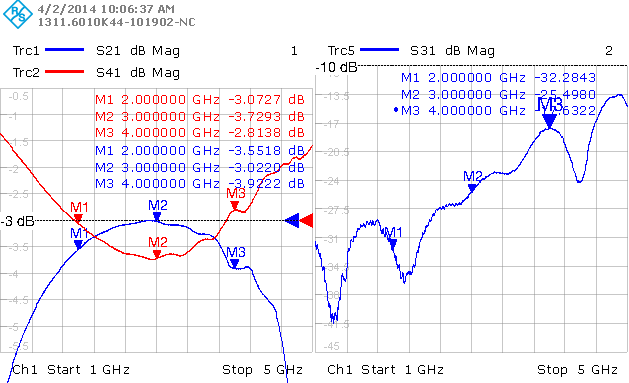
\includegraphics[width=\textwidth]{figures/network_analyzer/Meca_705S-3_coupler_id1}
  \caption{Measurements of Meca 3 dB Hybrid Coupler 705S-3.000,
    $x_1 \triangleq $ port 1, $y_1 \triangleq $ = port 2,
    $x_2 \triangleq $ port 3, $y_2 \triangleq $ = port 4}
  \label{fig:90deg_coupler_measurement}
\end{figure}

\begin{table}[h]
  \centering
  \begin{tabular}{|l|l|}
    \hline
    Operation range & 2 - 4 GHz \\ \hline
    Frequency Sensitivity & $\pm$ 0.4 dB \\ \hline
    Coupling variation & 3.1 dB $\pm$ 0.6 db \\ \hline
    Typical Isolation & 22 dB \\ \hline
    max \gls{VSWR} & 1.2 : 1 \\ \hline
    Phase rotation & $90^\circ \pm 2.0^\circ$ \\ \hline
  \end{tabular}
  \caption{Key properties of Meca 3 dB Hybrid Coupler 705S-3.000 \cite{meca_705s}}
  \label{tab:awg}
\end{table}

\section{Mini-Circuits Amplifier ZX60-V63+}
Whenever additional gain was needed to drive a mixer input or the \gls{ADC}
with the proper power level, power amplifiers made by Mini-Circuits were used. \\

It's key properties are shown in \tblref{tab:comp_zx60}, a picture is shown in
\figref{fig:comp_zx60_pic} and my own gain and \gls{VSWR} measurements are shown in
\figref{fig:comp_zx60_meas}. \\

\begin{table}
  \centering
  \begin{tabular}{|l|l|}
    \hline
    Operation range & 0.05 - 6 GHz \\ \hline
    Gain & 21.9 dB typ. at 0.05 GHz, 15.4 dB typ. at 6 GHz \\ \hline
    Flatness & $\pm$ 1.7 dB from 50 to 3000 MHz \\ \hline
    1 dB compression point (out. power) & min. 17 dBm \\ \hline
  \end{tabular}
  \caption{Key properties of Mini-Circuits Amplifier ZX60-V63+ \cite{mc_zx60}}
  \label{tab:comp_zx60}
\end{table}

\begin{figure}[p]
  \centering
  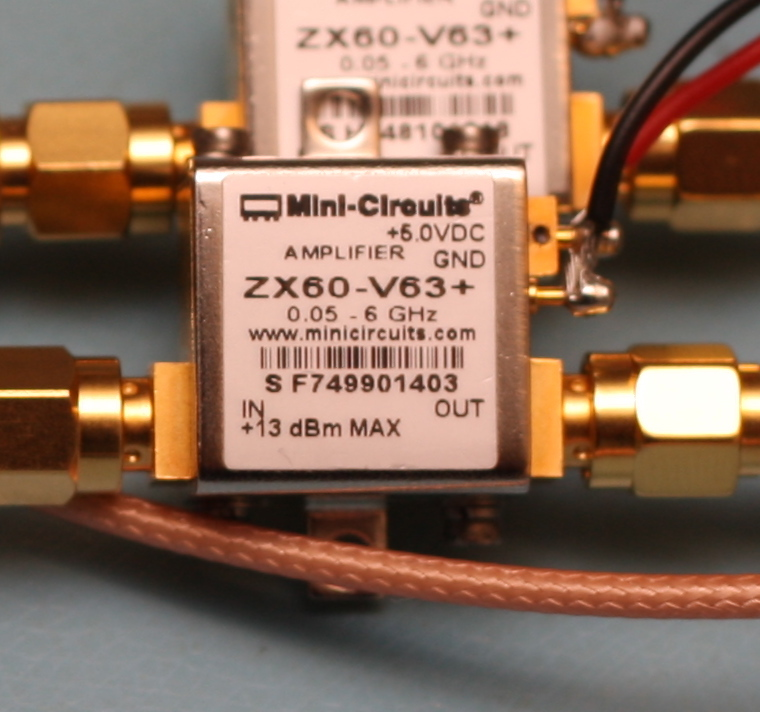
\includegraphics[width=0.4\textwidth]{pictures/ZX60-V63+}
  \caption{\gls{MC} Amplifier ZX60-V63+}
  \label{fig:comp_zx60_pic}
\end{figure}

\begin{figure}[p]
  \centering
  \begin{subfigure}{0.45\textwidth}
    \centering
    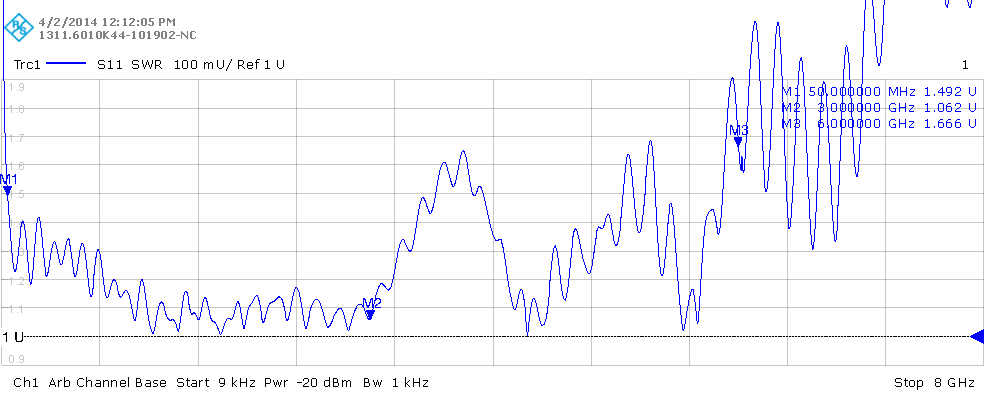
\includegraphics[width=\textwidth]{figures/network_analyzer/MCL_ZX60-V63+_Amplifier_S11_id1}
    \caption{\gls{VSWR} of the input}
  \end{subfigure}
  ~
  \begin{subfigure}{0.45\textwidth}
    \centering
    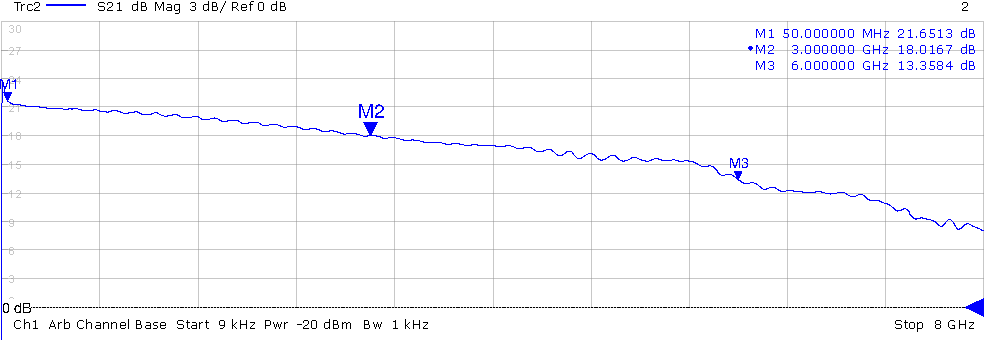
\includegraphics[width=\textwidth]{figures/network_analyzer/MCL_ZX60-V63+_Amplifier_S21_id1}
    \caption{Gain vs. Frequency}
  \end{subfigure}
  \caption{Measurements of Mini-Circuits Amplifier ZX60-V63+,
    input $\triangleq$ port 1, output $\triangleq$ port 2}
  \label{fig:comp_zx60_meas}
\end{figure}

\section{Mini-Circuits High-pass Filter BHP-1000+}
For the setup described in \chapref{chap:res_450}, a high-pass filter
by Mini-Circuits was as the lower bound for the channel selection filter.
It's properties are listed in \tblref{tab:comp_bhp1000} and a picture is given in
\figref{fig:comp_bhp1000_pic}.

\begin{table}
  \centering
  \begin{tabular}{|l|l|}
    \hline
    Stop Band ($\geq$3dB) & $<$ 0.9 GHz \\ \hline
    Pass Band ($<$ 1dB) & 1 - 3 GHz \\ \hline
  \end{tabular}
  \caption{Key properties of High-pass Filter BHP-1000+ \cite{mc_bhp1000}}
  \label{tab:comp_zx60}
\end{table}

\begin{figure}[p]
  \centering
  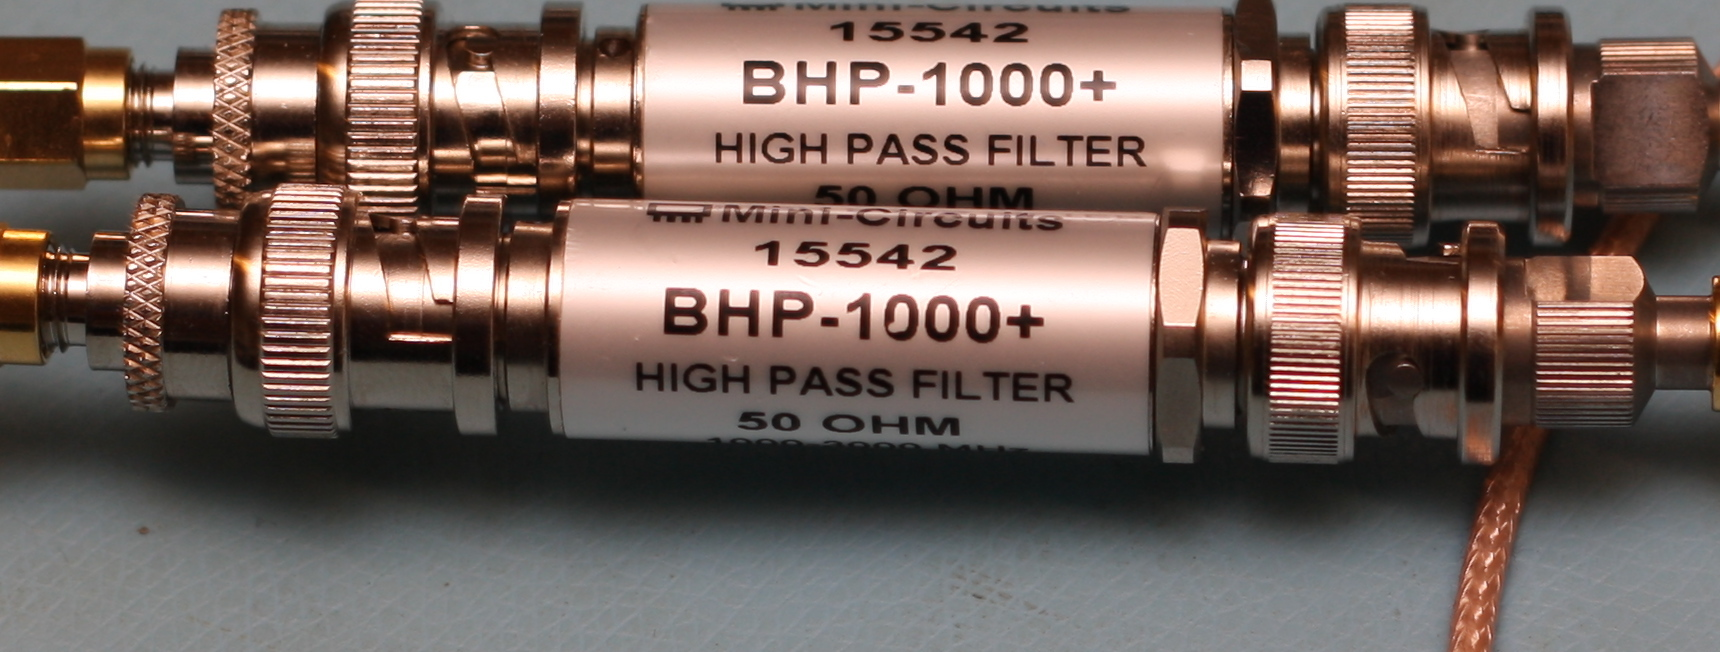
\includegraphics[width=0.4\textwidth]{pictures/BHP-1000+}
  \caption{High-pass Filter BHP-1000+}
  \label{fig:comp_bhp1000_pic}
\end{figure}

\section{Mini-Circuits DC Block MCL BLK-89-S+}
\label{sec:comp_dc_block}
To prevent \gls{DC} from driving amplifier inputs into saturation
a \gls{DC}-block was used. A significantly higher insertion loss was
measured than specified in the data sheet as shown in
\tblref{tab:comp_dc_block} and \figref{fig:comp_dc_block_insertion_loss}.

\begin{table}[h]
  \centering
  \begin{tabular}{|l|l|}
    \hline
    Pass Band & 0.1 MHz to 8 GHz \\ \hline
    Specified Insertion loss up to 4 GHz & $<$ 0.8 dB \\ \hline
    Measured Insertion loss up to 4 GHz & $<$ 0.8 dB \\ \hline
  \end{tabular}
  \caption{Key properties of Mini-Circuits DC Block MCL BLK-89-S+ \cite{mc_blk89}}
  \label{tab:comp_dc_block}
\end{table}

\begin{figure}[p]
  \centering
  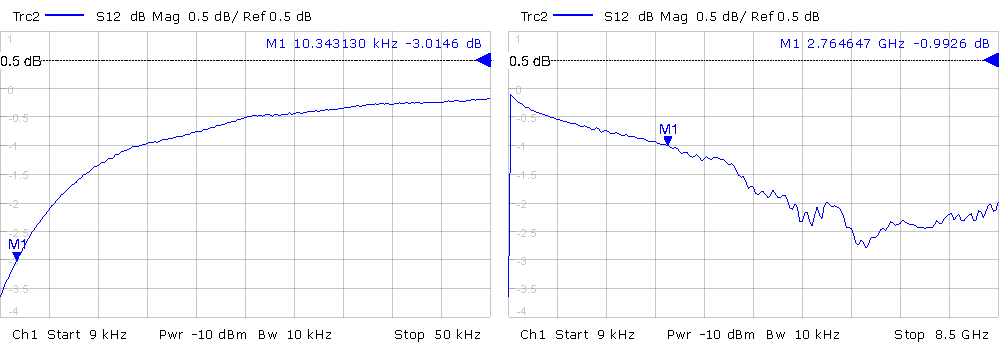
\includegraphics[width=\textwidth]{figures/network_analyzer/MCL_BLK-89-S+_DC-Block_insertion_loss}
  \caption{Measured Insertion Loss of Mini-Circuits DC Block MCL BLK-89-S+}
  \label{fig:comp_dc_block_insertion_loss}
\end{figure}

\section{Mini-Circuits Attenuators VAT+}
\label{sec:comp_vat}
To adjust all the power levels across the \gls{RF} part, fixed
attenuators were used. The 1 dB version is shown in
\figref{fig:comp_vat_pic}. \tblref{tab:comp_vat} shown the key properties
of these attenuators.

\begin{table}[h]
  \centering
  \begin{tabular}{|l|l|}
    \hline
    Operation range & DC - 6 GHz \\ \hline
  \end{tabular}
  \caption{Key property of Mini-Circuits Attenuators VAT+ \cite{mc_vat1}}
  \label{tab:comp_dc_block}
\end{table}

\begin{figure}[p]
  \centering
  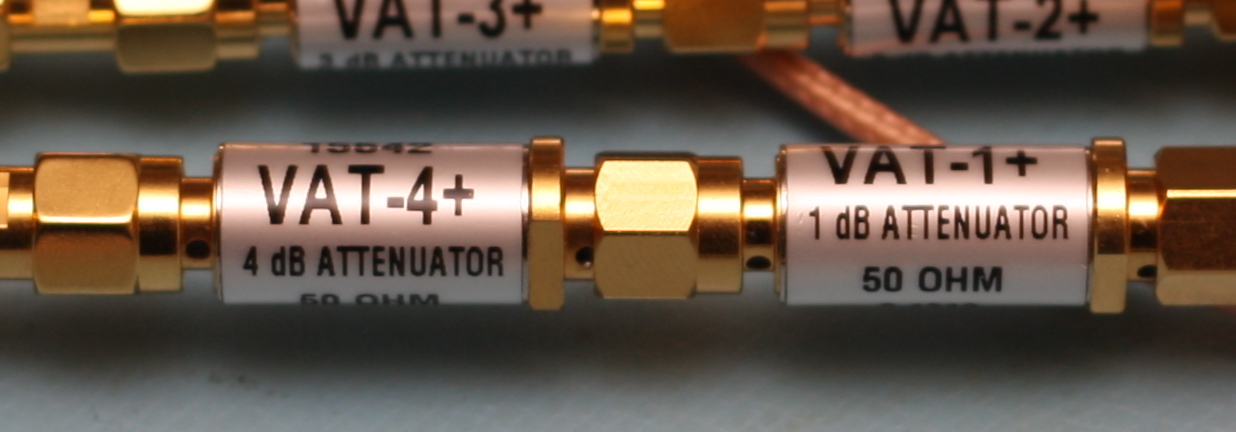
\includegraphics[width=0.4\textwidth]{pictures/attenuator}
  \caption{\gls{MC} attenuators}
  \label{fig:comp_vat_pic}
\end{figure}

\section{Texas-Instruments Baluns ADC-WB-BB and ADC-LB-BB}
\label{sec:comp_balun}
The received \gls{IF} signals are single ended and the impedance of all
components and cables is 50 $\Omega$. The \gls{ADC} on the other hand, uses
differential inputs with an impedance of 100 $\Omega$. Therefor baluns are used
for conversion. The \gls{VSWR} and insertion loss measurements of the used
ADC-WB-BB are shown in \figref{fig:comp_wbbb}. The ADC-LB-BB, which was also
available was not used due to it's high insertion loss at low frequencies. \\

\begin{figure}[p]
  \centering
  \begin{subfigure}{0.45\textwidth}
    \centering
    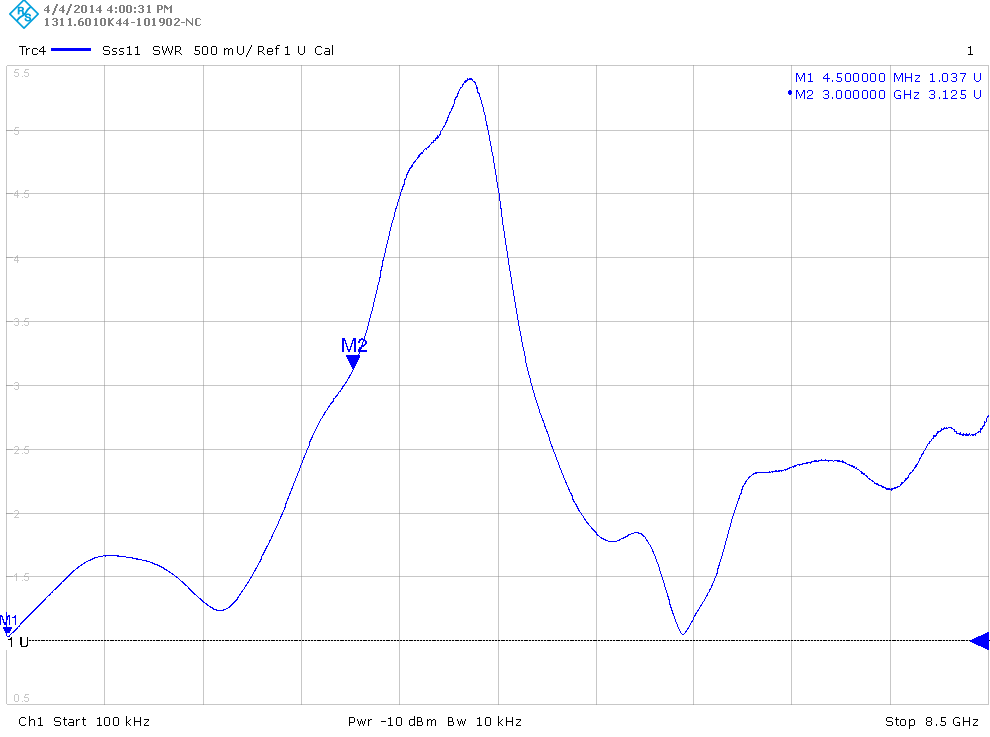
\includegraphics[width=\textwidth]{figures/network_analyzer/TI_ADC-WB-BB_Balun_swr_id1}
    \caption{\gls{VSWR} of the input}
  \end{subfigure}
  ~
  \begin{subfigure}{0.45\textwidth}
    \centering
    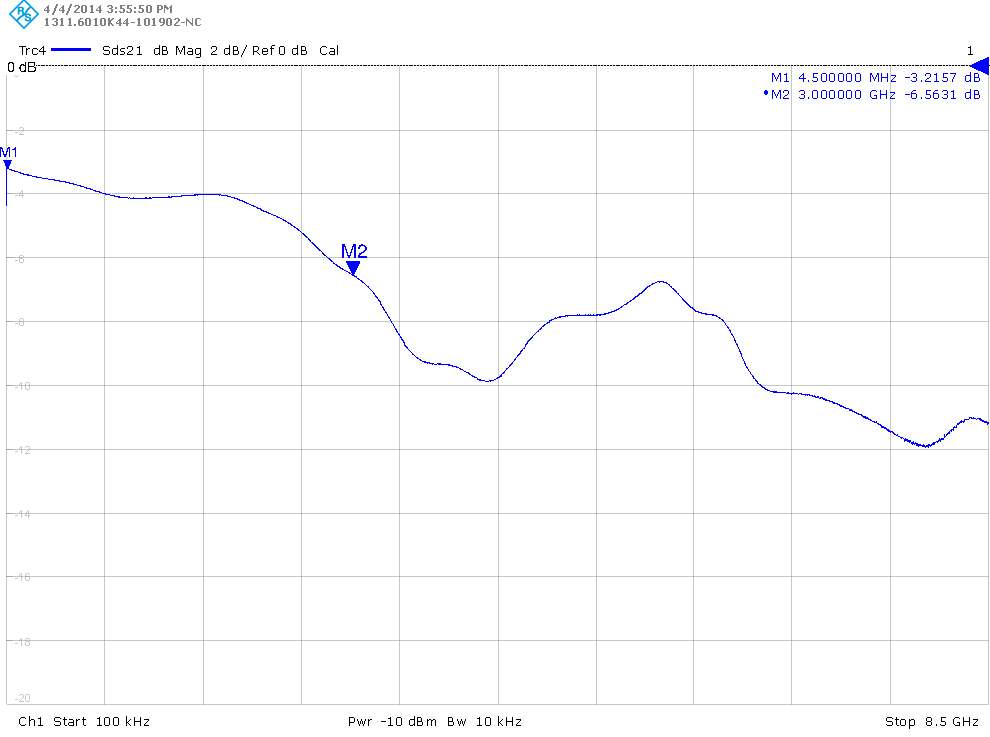
\includegraphics[width=\textwidth]{figures/network_analyzer/TI_ADC-WB-BB_Balun_insertion_loss_id1}
    \caption{Insertion Loss}
  \end{subfigure}
  \caption{Measurements of Texas-Instruments Balun ADC-WB-BB,
    input $\triangleq$ port 1, output $\triangleq$ port 2}
  \label{fig:comp_wbbb}
\end{figure}

\begin{figure}[p]
  \centering
  \begin{subfigure}{0.45\textwidth}
    \centering
    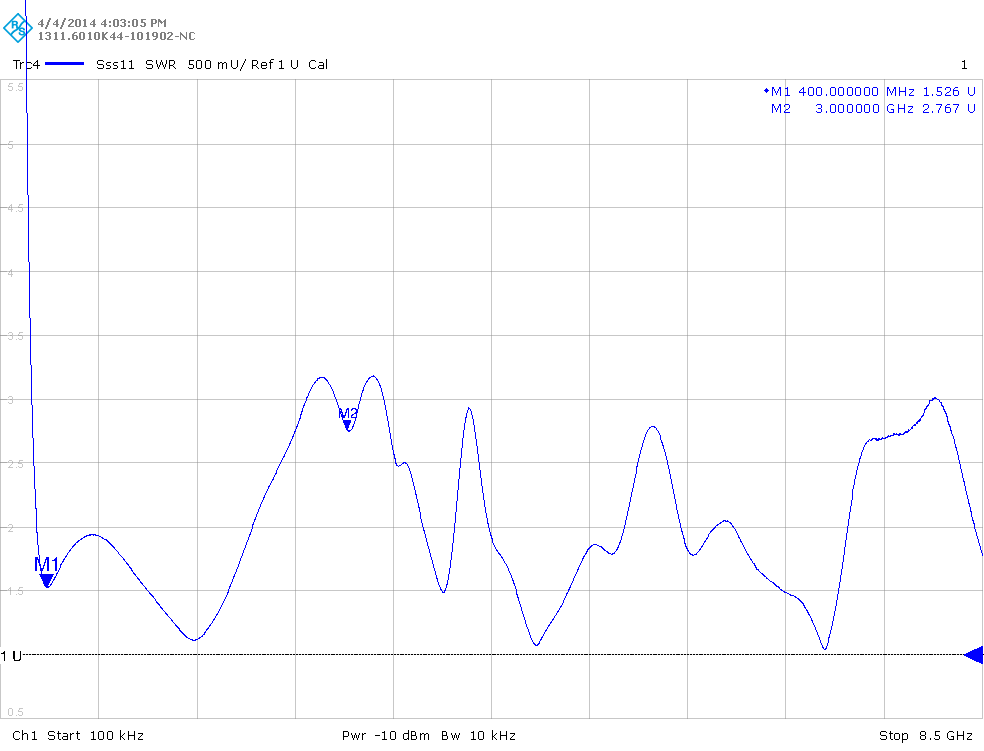
\includegraphics[width=\textwidth]{figures/network_analyzer/TI_ADC-LB-BB_Balun_swr_id1}
    \caption{\gls{VSWR} of the input}
  \end{subfigure}
  ~
  \begin{subfigure}{0.45\textwidth}
    \centering
    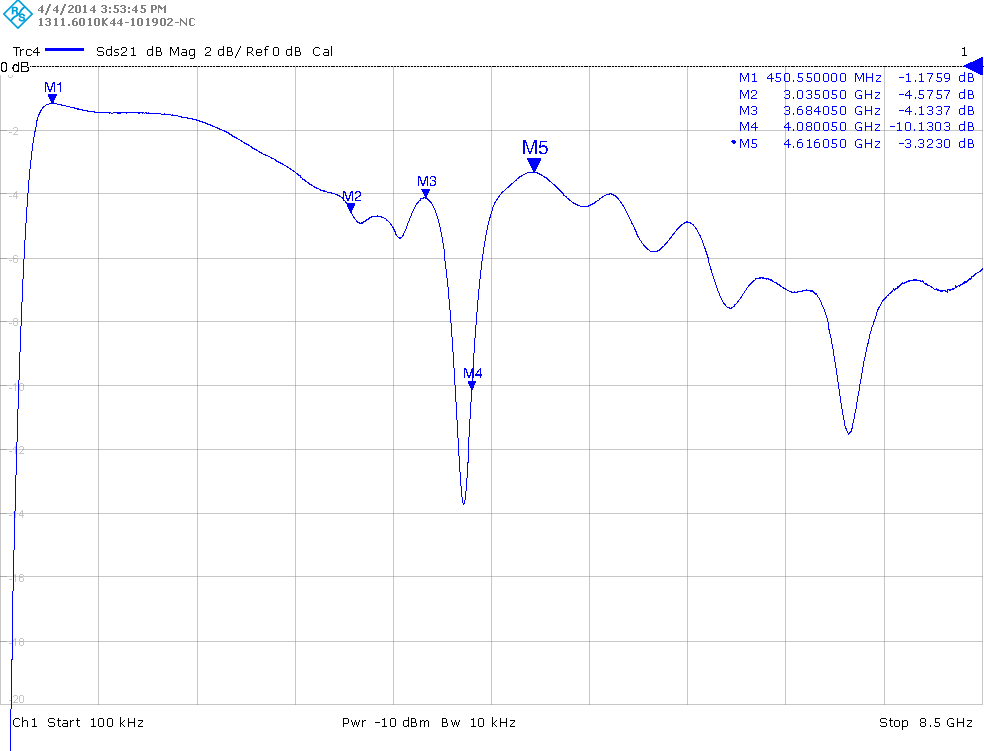
\includegraphics[width=\textwidth]{figures/network_analyzer/TI_ADC-LB-BB_Balun_insertion_loss_id1}
    \caption{Insertion Loss}
  \end{subfigure}
  \caption{Measurements of Texas-Instruments Balun ADC-LB-BB,
    input $\triangleq$ port 1, output $\triangleq$ port 2}
  \label{fig:comp_lbbb}
\end{figure}

\begin{figure}[p]
  \centering
  %\includegraphics[width=0.4\textwidth]{pictures/}
  \caption{Picture of Texas-Instruments Balun ADC-WB-BB}
  \label{fig:comp_balun_pic}
\end{figure}

\section{Texas Instruments ADC 12d1800}
\label{sec:comp_adc}
The receiver was build using the Ultra High-Speed ADC12D1800 by Texas Instruments.
It is able to either sample two channels at 1.8 $\text{GS}/\text{s}$ or to interleave
this two channels by applying the same input signal to both channels and sampling
one on the positive and the other one on the negative clock edge resulting in sample
rates of up to 3.6 $\text{GS}/\text{s}$. The vertical resolution of 12 bits is better
than the one of the used oscilloscope (\secref{sec:comp_osci}) and in most scenarios
not the \gls{SNR} limiting factor even when the signal is 6 db below full-scale.
The huge analog bandwidth of about 100 kHz
(limited by the \gls{DC} block described in \secref{sec:comp_dc_block}) to about
2.8 GHz allows to not only sample the first Nyquist-zone but also allows
for sub-sampling which was particular interest. \\

The ADC12D1800 Reference Board was used which has a very well optimized board
layout, supports \gls{SMA} plugs for all important signals, includes a
\gls{FPGA} and \gls{USB} interface for configuration and a power supply.
The reference board has an on-board \gls{PLL} but was often clocked by a marker
output of the \gls{AWG}.
An \gls{FMC} connector exposes the full interface of the \gls{ADC} to
the on board \gls{FPGA} and is used by the Virtex-7 board to capture the data
as described in \chapref{chap:fpga}. \\

\begin{table}[h]
  \centering
  \begin{tabular}{|l|l|}
    \hline
    Number of channels & 2, 1 interleaved \\ \hline
    Sample Rate & $\leq$ 1.8 $\text{GS}/\text{s}$, $\leq$ 3.6 $\text{GS}/\text{s}$ interleaved \\ \hline
    Analog Bandwidth & typical 2.8 GHz \\ \hline
    Vertical Resolution & 12 bit \\ \hline
    Noise Floor Density & $\approx$ -150 $\text{dB}/\text{Hz}$ \\ \hline
    Power Consumption & 4.7 W \\ \hline
  \end{tabular}
  \caption{Key properties of Texas-Instruments ADC 12d1800 \cite{ti_adc12d1800}}
  \label{tab:comp_adc}
\end{table}

\section{Xilinx Virtex 7 Board VC707}
\label{sec:comp_vc707}
For the data acquisition and storage the VC707 Virtex-7 evaluation board
was used. It's key features are listed in \tblref{tab:comp_vc707} and a
picture is shown in \figref{fig:comp_vc707_pic}.


\begin{table}[h]
  \centering
  \begin{tabular}{|l|l|}
    \hline
    Bit-File Storage & 128 MB Linear byte peripheral interface (BPI) Flash memory \\ \hline
    Download-Interface & USB 2.0 ULPI Transceiver \\ \hline
    Program \& Debug Interface & USB JTAG through Digilent module \\ \hline
    User I/O & 5 Push-Buttons, 4 GPIO SMA plugs \\ \hline
    Connection to \gls{ADC} board & VITA 57.1 FMC1 HPC Connector \\ \hline
    Logic Cells & 85'760 \\ \hline
    Block RAM Size &  37'080 kB \\ \hline
    Total I/O Banks & 14 \\ \hline
  \end{tabular}
  \caption{Relevant properties of Xilinx Virtex 7 Evaluation Board VC707
    \cite{xilinx_virtex7_overview, xilinx_vc707}}
  \label{tab:comp_vc707}
\end{table}

\begin{figure}[p]
  \centering
  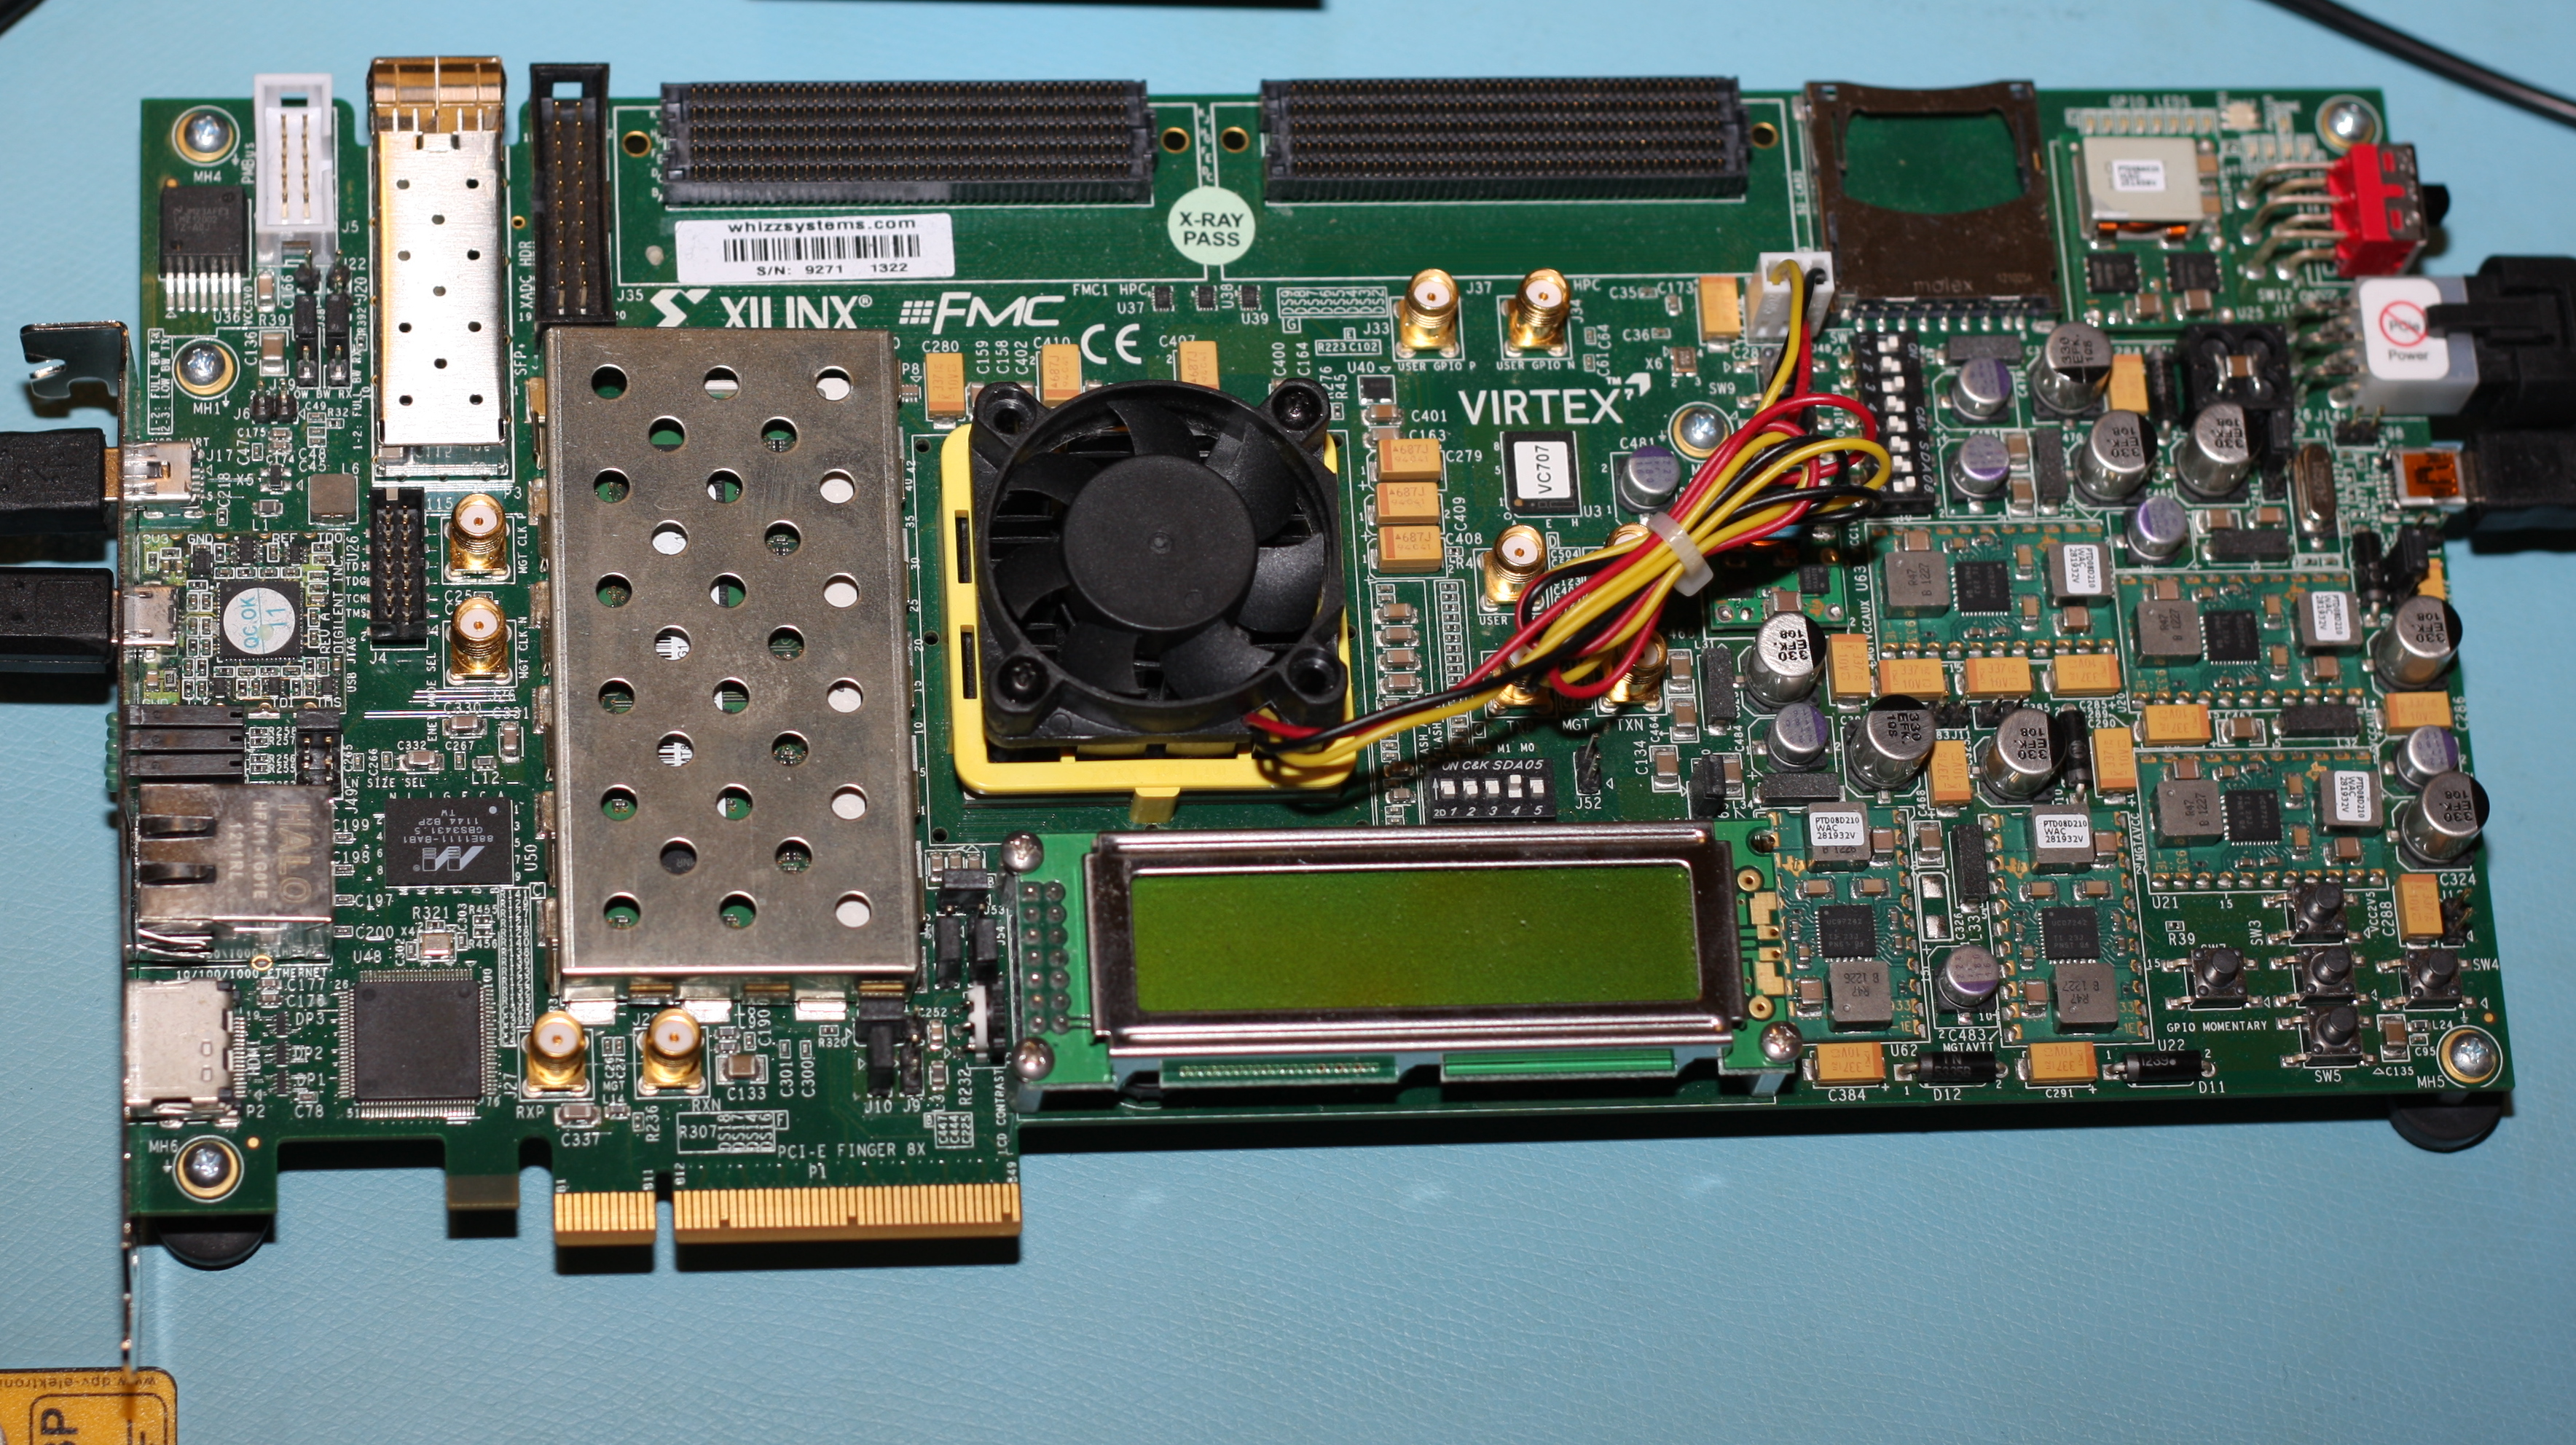
\includegraphics[width=\textwidth]{pictures/vc707}
  \caption{Picture of Xilinx Virtex 7 Evaluation Board VC707}
  \label{fig:comp_vc707_pic}
\end{figure}

\section{R\&S Oscilloscope RTO 1044}
\label{sec:comp_osci}
High frequency measurements were made on a Rohde \& Schwarz Digital
Oscilloscope RTO 1044. With the optional reference input it could be locked
to the \gls{AWG} as well used to have a very precise ($\pm 0.02 \text{ppm}$),
oven controlled 10 MHz reference. \\

During many experiments the real time \gls{FFT} display of the oscilloscope was
proven very useful to check power levels and signal shapes. \\

Since the VISA standard for instrument control is painful to install under
Redhat 6 a small program based on the VXI-11 library written by
Steve D. Sharples\footnote{see: http://optics.eee.nottingham.ac.uk/vxi11/}
was written to convert simple telnet commands send by Matlab
to remote procedure calls. This allowed to setup and readout the oscilloscope
directly in the Matlab simulation framework. This was used to do first experiments
on the actual \gls{RF} hardware before the \gls{FPGA} (\chapref{chap:fpga}) was
completely implemented. \\

\begin{table}[h]
  \centering
  \begin{tabular}{|l|l|}
    \hline
    Number of channels & 4, 2 interleaved \\ \hline
    Sample Rate & 10 $\text{GS}/\text{s}$, 20 $\text{GS}/\text{s}$ interleaved \\ \hline
    Analog Bandwidth at 50 $\Omega$ & $\geq 4$ GHz \\ \hline
    Vertical Resolution & 8 bit \\ \hline
  \end{tabular}
  \caption{Key properties of R\&S Oscilloscope RTO 1044}
  \label{tab:awg}
\end{table}

%%  LocalWords:  datasheets ZNB idealities Rohde Schwarz overbended
%%  LocalWords:  dBs Tektronix AWG Matlab baseband FPGA Sivers IMA FC
%%  LocalWords:  PLL sivers coupler USBand LSBand LSB ima dBm Meca WB
%%  LocalWords:  VSWR Balun MCL BLK osci SNR Nyquist SMA FMC Virtex
%%  LocalWords:  fpga Xilinx VC RTO FFT Redhat VXI Sharples rx rf ZX
%%  LocalWords:  zx typ BHP bhp Attenuators attenuators Baluns baluns
%%  LocalWords:  wbbb vc BPI ULPI JTAG Digilent GPIO HPC kB
